In this section we document the results on the $WW$ cross-section 
measurement. In this measurement we apply the same event 
selection as in the HWW search at the WW level 
(see Section~\ref{sec:selection}  with the 
additional selection on the trailing lepton pT greater than 20 GeV. 

\subsection{Background Estimations}

Table~\ref{tab:dy_wwxec}-\ref{tab:ttbar_xsec} shows the Drell-Yan and Top 
background estimations for the $WW$ cross-section measurements. 

%%%%%%%%%%%%%%%%%%%%%%%%%%%%%%
\begin{table}[ht!]
\begin{center}
\begin{tabular}{c c c c c c}
\hline
       nJets & $N_{in}$(data)        & $R_{out/in}$        & $N_{out}$(data)  & $N_{out}$ (MC) \\ 
\hline
0 & 377.1$\pm$46.8 & 0.20$\pm$0.01$\pm$0.01 & 73.6$\pm$10.1$\pm$4.7 & 13.68$\pm$4.90 \\
1 & 171.7$\pm$25.5 & 0.18$\pm$0.01$\pm$0.01 & 30.3$\pm$4.7$\pm$2.0  & 11.70$\pm$4.56 \\
2 & 1755.4$\pm$46.1 & 0.20$\pm$0.01$\pm$0.01 & 359.2$\pm$16.9$\pm$12.7  & 175.79$\pm$16.76 \\
\hline
\end{tabular}
\caption{The Drell-Yan estimation in the same flavor final state for WW cross-section measurements, 
using the DYMVA in 0 and 1 Jet bins and the pfMET at the 2-jet bins. }
\label{tab:dy_wwxec}
\end{center}
\end{table}
%%%%%%%%%%%%%%%%%%%%%%%%%%%%%%


%%%%%%%%%%%%%%%%%%%%%%%%%%%%%%
\begin{table}[ht!]
\begin{center}
\begin{tabular}{l c c c}
\hline
                                   Sample & 0-jet           & 1-jet           & 2-jet       \\
\hline
estimated top events in simulation  & 361.8 $\pm$  7.4 &  1121.7 $\pm$  11.7 &  1343.4 $\pm$ 9.6 \\
tagging efficiency     (\%)         & 49.6 $\pm$  4.3 & 65.1 $\pm$  0.6 & - \\ 
data events in control region       &  496 & 2502 & - \\ 
background events in control region & 133.9 $\pm$  30.1 &  133.5 $\pm$  30.0 & - \\ 
top estimation in data              & 367.8 $\pm$  54.5 &  1204.7 $\pm$  46.5 &   1571.2 $\pm$ 63.2 \\
data/simulation scale factor        & 1.02 $\pm$  0.15 &   1.07 $\pm$  0.04 &  1.17 $\pm$  0.05 \\

\hline
\end{tabular}
\caption{Monte Carlo to data scale factor for the top background contribution for $\intlumiEightTeV$. 
In the 1-jet bin, the scale factor is derived in a region that is slightly different from the signal region.}
\label{tab:ttbar_xsec}
\end{center}
\end{table}
%%%%%%%%%%%%%%%%%%%%%%%%%%%%%%


\subsection{Results in Zero jet bin}

\begin{table}[!ht]
{\small
\begin{center}
\begin{tabular}{|l|c|c|c|c|}
\hline
Sample	& mm	& me	& em	& ee	\\ \hline
$qqWW$	& $498.48 \pm 4.72 \pm 36.09 $	& $617.76 \pm 5.13 \pm 43.54 $	& $734.35 \pm 5.62 \pm 51.75 $	& $309.84 \pm 3.64 \pm 23.88 $	\\ 
$qqWW$	& $32.97 \pm 0.90 \pm 10.14 $	& $36.82 \pm 0.93 \pm 11.30 $	& $44.56 \pm 1.03 \pm 13.68 $	& $22.39 \pm 0.73 \pm 6.91 $	\\ 
$t\bar{t} + tW$	& $82.26 \pm 3.63 \pm 12.34 $	& $107.42 \pm 4.00 \pm 16.11 $	& $128.67 \pm 4.42 \pm 19.30 $	& $50.64 \pm 2.82 \pm 7.60 $	\\ 
$W+jets$	& $31.49 \pm 5.91 \pm 11.34 $	& $38.07 \pm 4.05 \pm 13.70 $	& $86.90 \pm 6.27 \pm 31.29 $	& $34.85 \pm 2.21 \pm 12.55 $	\\ 
$WZ$	& $19.55 \pm 0.39 \pm 2.16 $	& $13.49 \pm 0.32 \pm 1.47 $	& $21.71 \pm 0.40 \pm 2.37 $	& $10.18 \pm 0.27 \pm 1.16 $	\\ 
$ZZ$	& $16.79 \pm 0.30 \pm 1.60 $	& $0.87 \pm 0.05 \pm 0.08 $	& $1.45 \pm 0.06 \pm 0.14 $	& $9.83 \pm 0.23 \pm 0.97 $	\\ 
$Z/\gamma*$	& $21.53 \pm 14.42 \pm 1.38 $	& $2.90 \pm 2.06 \pm 0.29 $	& $0.24 \pm 0.24 \pm 0.02 $	& $52.06 \pm 22.10 \pm 3.32 $	\\ 
$W\gamma*/W+\gamma$	& $2.88 \pm 0.71 \pm 0.86 $	& $12.03 \pm 3.37 \pm 3.61 $	& $25.63 \pm 4.73 \pm 7.69 $	& $49.46 \pm 5.46 \pm 14.84 $	\\ 
\hline \hline 
Total B.	& $174.51 \pm 16.02 \pm 17.05 $	& $174.78 \pm 6.93 \pm 21.51 $	& $264.60 \pm 9.03 \pm 37.63 $	& $207.02 \pm 23.04 \pm 21.18 $	\\ \hline \hline 
Total B.+S.	& $705.95 \pm 16.73 \pm 41.18 $	& $829.35 \pm 8.68 \pm 49.86 $	& $1043.50 \pm 10.69 \pm 65.43 $	& $539.24 \pm 23.34 \pm 32.66 $	\\ \hline \hline
Data	& $850$ 	& $956$ 	& $1217$ 	& $558$ 	\\ \hline \hline
Acceptance ( \% )	& $0.73 \pm 0.06 	$& $0.90 \pm 0.07 	$& $1.07 \pm 0.08 	$& $0.46 \pm 0.04 	$\\ 
Cross Section ( pb )	& $72.59 \pm 3.13 \pm 6.29$ 	& $68.16 \pm 2.70 \pm 5.64$ 	& $69.83 \pm 2.56 \pm 6.12$ 	& $60.33 \pm 4.06 \pm 7.39$ 	\\ \hline
\end{tabular}
\caption{Summary of yields for 0-jet channel.Uncertainties on yields and cross sections are $\mathrm{(stat.)} \pm \mathrm{(syst.)}$.The systematic uncertainty on the cross section does not include the luminosity}
\label{tab:datayields_wwxsec_0j}
\end{center}}
\end{table}
\begin{table}[!ht]
{\small
\begin{center}
\begin{tabular}{|l|c|c|c|c|}
\hline
Sample	& incl	\\ \hline
$qqWW$	& $2160.42 \pm 9.67 \pm 155.27 $	\\ 
$qqWW$	& $136.73 \pm 1.81 \pm 42.03 $	\\ 
$t\bar{t} + tW$	& $368.99 \pm 7.53 \pm 55.35 $	\\ 
$W+jets$	& $191.31 \pm 9.78 \pm 68.87 $	\\ 
$WZ$	& $64.93 \pm 0.70 \pm 7.17 $	\\ 
$ZZ$	& $28.94 \pm 0.38 \pm 2.79 $	\\ 
$Z/\gamma*$	& $76.74 \pm 26.46 \pm 4.71 $	\\ 
$W\gamma*/W+\gamma$	& $89.99 \pm 8.01 \pm 27.00 $	\\ 
\hline \hline 
Total B.	& $820.90 \pm 30.29 \pm 92.83 $	\\ \hline \hline 
Total B.+S.	& $3118.05 \pm 31.84 \pm 185.72 $	\\ \hline \hline
Data	& $3581$ 	\\ \hline \hline
Acceptance ( \% )	& $3.17 \pm 0.25 	$\\ 
Cross Section ( pb )	& $68.62 \pm 1.49 \pm 5.94$ 	\\ \hline
\end{tabular}
\caption{Summary of yields for 0-jet channel.Uncertainties on yields and cross sections are $\mathrm{(stat.)} \pm \mathrm{(syst.)}$.The systematic uncertainty on the cross section does not include the luminosity}
\label{tab:datayields_wwxsec_0j}
\end{center}}
\end{table}
\clearpage


\subsection{Results in One jet bin}

\begin{table}[!ht]
{\small
\begin{center}
\begin{tabular}{|l|c|c|c|c|}
\hline
Sample	& mm	& me	& em	& ee	\\ \hline
$qqWW$	& $161.92 \pm 2.69 \pm 11.72 $	& $268.99 \pm 3.37 \pm 18.96 $	& $319.65 \pm 3.72 \pm 22.53 $	& $101.67 \pm 2.08 \pm 7.84 $	\\ 
$qqWW$	& $10.15 \pm 0.50 \pm 3.12 $	& $15.48 \pm 0.60 \pm 4.75 $	& $18.27 \pm 0.66 \pm 5.61 $	& $7.01 \pm 0.42 \pm 2.16 $	\\ 
$t\bar{t} + tW$	& $215.28 \pm 5.03 \pm 8.61 $	& $345.67 \pm 6.50 \pm 13.83 $	& $398.60 \pm 7.06 \pm 15.94 $	& $135.05 \pm 3.92 \pm 5.40 $	\\ 
$W+jets$	& $29.53 \pm 5.55 \pm 10.63 $	& $44.36 \pm 4.78 \pm 15.97 $	& $98.17 \pm 6.93 \pm 35.34 $	& $15.26 \pm 1.56 \pm 5.49 $	\\ 
$WZ$	& $9.47 \pm 0.27 \pm 1.05 $	& $16.88 \pm 0.35 \pm 1.84 $	& $26.57 \pm 0.45 \pm 2.90 $	& $9.29 \pm 0.26 \pm 1.06 $	\\ 
$ZZ$	& $4.98 \pm 0.16 \pm 0.47 $	& $0.98 \pm 0.05 \pm 0.09 $	& $1.62 \pm 0.06 \pm 0.15 $	& $3.21 \pm 0.13 \pm 0.32 $	\\ 
$Z/\gamma*$	& $26.92 \pm 11.30 \pm 1.78 $	& $19.55 \pm 5.71 \pm 1.96 $	& $31.52 \pm 7.26 \pm 3.15 $	& $3.39 \pm 3.39 \pm 0.22 $	\\ 
$W\gamma*/W+\gamma$	& $0.00 \pm 0.00 \pm 0.00 $	& $3.99 \pm 1.44 \pm 1.20 $	& $16.27 \pm 4.48 \pm 4.88 $	& $19.97 \pm 3.63 \pm 5.99 $	\\ 
\hline \hline 
Total B.	& $286.18 \pm 13.56 \pm 13.84 $	& $431.44 \pm 10.00 \pm 21.33 $	& $572.75 \pm 13.07 \pm 39.31 $	& $186.16 \pm 6.53 \pm 9.82 $	\\ \hline \hline 
Total B.+S.	& $458.24 \pm 13.83 \pm 18.41 $	& $715.90 \pm 10.57 \pm 28.93 $	& $910.68 \pm 13.61 \pm 45.66 $	& $294.84 \pm 6.86 \pm 12.75 $	\\ \hline \hline
Data	& $468$ 	& $720$ 	& $960$ 	& $292$ 	\\ \hline \hline
Acceptance ( \% )	& $0.24 \pm 0.02 	$& $0.39 \pm 0.03 	$& $0.47 \pm 0.04 	$& $0.15 \pm 0.01 	$\\ 
Cross Section ( pb )	& $60.35 \pm 7.18 \pm 8.02$ 	& $57.93 \pm 5.39 \pm 6.52$ 	& $65.45 \pm 5.24 \pm 8.65$ 	& $55.62 \pm 8.98 \pm 7.76$ 	\\ \hline
\end{tabular}
\caption{Summary of yields for 1-jet channel.Uncertainties on yields and cross sections are $\mathrm{(stat.)} \pm \mathrm{(syst.)}$.The systematic uncertainty on the cross section does not include the luminosity}
\label{tab:datayields_wwxsec_1j}
\end{center}}
\end{table}
\begin{table}[!ht]
{\small
\begin{center}
\begin{tabular}{|l|c|c|c|c|}
\hline
Sample	& incl	\\ \hline
$qqWW$	& $852.22 \pm 6.06 \pm 61.05 $	\\ 
$qqWW$	& $50.91 \pm 1.10 \pm 15.65 $	\\ 
$t\bar{t} + tW$	& $1094.61 \pm 11.52 \pm 43.78 $	\\ 
$W+jets$	& $187.32 \pm 10.20 \pm 67.43 $	\\ 
$WZ$	& $62.20 \pm 0.68 \pm 6.85 $	\\ 
$ZZ$	& $10.79 \pm 0.23 \pm 1.03 $	\\ 
$Z/\gamma*$	& $81.38 \pm 14.98 \pm 5.48 $	\\ 
$W\gamma*/W+\gamma$	& $40.23 \pm 5.95 \pm 12.07 $	\\ 
\hline \hline 
Total B.	& $1476.53 \pm 22.30 \pm 81.78 $	\\ \hline \hline 
Total B.+S.	& $2379.66 \pm 23.14 \pm 103.25 $	\\ \hline \hline
Data	& $2440$ 	\\ \hline \hline
Acceptance ( \% )	& $1.24 \pm 0.10 	$\\ 
Cross Section ( pb )	& $60.93 \pm 3.12 \pm 7.19$ 	\\ \hline
\end{tabular}
\caption{Summary of yields for 1-jet channel.Uncertainties on yields and cross sections are $\mathrm{(stat.)} \pm \mathrm{(syst.)}$.The systematic uncertainty on the cross section does not include the luminosity}
\label{tab:datayields_wwxsec_1j}
\end{center}}
\end{table}
\clearpage
\subsection{Rseults in Two jet bin}

\begin{table}[!ht]
{\small
\begin{center}
\begin{tabular}{|l|c|c|c|c|}
\hline
Sample	& mm	& me	& em	& ee	\\ \hline
$qqWW$	& $80.14 \pm 1.88 \pm 5.80 $	& $111.55 \pm 2.17 \pm 7.86 $	& $126.48 \pm 2.35 \pm 8.91 $	& $51.28 \pm 1.47 \pm 3.95 $	\\ 
$qqWW$	& $2.21 \pm 0.23 \pm 0.68 $	& $3.16 \pm 0.27 \pm 0.97 $	& $3.62 \pm 0.29 \pm 1.11 $	& $1.54 \pm 0.19 \pm 0.48 $	\\ 
$t\bar{t} + tW$	& $356.78 \pm 5.42 \pm 17.84 $	& $464.41 \pm 6.11 \pm 23.22 $	& $536.47 \pm 6.49 \pm 26.82 $	& $214.15 \pm 4.07 \pm 10.71 $	\\ 
$W+jets$	& $24.34 \pm 6.75 \pm 8.76 $	& $29.78 \pm 4.34 \pm 10.72 $	& $61.97 \pm 6.15 \pm 22.31 $	& $13.39 \pm 1.54 \pm 4.82 $	\\ 
$WZ$	& $7.68 \pm 0.24 \pm 0.85 $	& $9.12 \pm 0.26 \pm 1.00 $	& $13.29 \pm 0.32 \pm 1.45 $	& $7.25 \pm 0.23 \pm 0.82 $	\\ 
$ZZ$	& $3.07 \pm 0.16 \pm 0.29 $	& $0.59 \pm 0.07 \pm 0.05 $	& $0.81 \pm 0.06 \pm 0.08 $	& $1.75 \pm 0.10 \pm 0.17 $	\\ 
$Z/\gamma*$	& $254.52 \pm 29.05 \pm 9.00 $	& $17.83 \pm 5.38 \pm 1.78 $	& $13.67 \pm 4.54 \pm 1.37 $	& $104.10 \pm 18.06 \pm 3.68 $	\\ 
$W\gamma*/W+\gamma$	& $0.15 \pm 0.15 \pm 0.04 $	& $2.99 \pm 2.58 \pm 0.90 $	& $2.92 \pm 1.92 \pm 0.88 $	& $1.84 \pm 0.82 \pm 0.55 $	\\ 
\hline \hline 
Total B.	& $646.54 \pm 30.31 \pm 21.84 $	& $524.72 \pm 9.58 \pm 25.67 $	& $629.14 \pm 10.21 \pm 34.96 $	& $342.48 \pm 18.59 \pm 12.35 $	\\ \hline \hline 
Total B.+S.	& $728.89 \pm 30.37 \pm 22.60 $	& $639.44 \pm 9.83 \pm 26.87 $	& $759.24 \pm 10.48 \pm 36.09 $	& $395.30 \pm 18.65 \pm 12.97 $	\\ \hline \hline
Data	& $704$ 	& $609$ 	& $790$ 	& $410$ 	\\ \hline \hline
Acceptance ( \% )	& $0.11 \pm 0.01 	$& $0.16 \pm 0.01 	$& $0.18 \pm 0.01 	$& $0.07 \pm 0.01 	$\\ 
Cross Section ( pb )	& $39.85 \pm 18.40 \pm 26.10$ 	& $41.96 \pm 12.29 \pm 14.03$ 	& $70.61 \pm 12.34 \pm 16.90$ 	& $73.01 \pm 21.89 \pm 24.90$ 	\\ \hline
\end{tabular}
\caption{Summary of yields for 2-jet channel.Uncertainties on yields and cross sections are $\mathrm{(stat.)} \pm \mathrm{(syst.)}$.The systematic uncertainty on the cross section does not include the luminosity}
\label{tab:datayields_wwxsec_2j}
\end{center}}
\end{table}
\begin{table}[!ht]
{\small
\begin{center}
\begin{tabular}{|l|c|c|c|c|}
\hline
Sample	& incl	\\ \hline
$qqWW$	& $369.46 \pm 3.99 \pm 26.53 $	\\ 
$qqWW$	& $10.53 \pm 0.50 \pm 3.24 $	\\ 
$t\bar{t} + tW$	& $1571.82 \pm 11.20 \pm 78.59 $	\\ 
$W+jets$	& $129.49 \pm 10.22 \pm 46.62 $	\\ 
$WZ$	& $37.33 \pm 0.53 \pm 4.12 $	\\ 
$ZZ$	& $6.22 \pm 0.21 \pm 0.60 $	\\ 
$Z/\gamma*$	& $390.11 \pm 34.92 \pm 13.06 $	\\ 
$W\gamma*/W+\gamma$	& $7.90 \pm 3.32 \pm 2.37 $	\\ 
\hline \hline 
Total B.	& $2142.88 \pm 38.22 \pm 92.43 $	\\ \hline \hline 
Total B.+S.	& $2522.87 \pm 38.43 \pm 96.22 $	\\ \hline \hline
Data	& $2513$ 	\\ \hline \hline
Acceptance ( \% )	& $0.52 \pm 0.04 	$\\ 
Cross Section ( pb )	& $55.63 \pm 7.53 \pm 15.66$ 	\\ \hline
\end{tabular}
\caption{Summary of yields for 2-jet channel.Uncertainties on yields and cross sections are $\mathrm{(stat.)} \pm \mathrm{(syst.)}$.The systematic uncertainty on the cross section does not include the luminosity}
\label{tab:datayields_wwxsec_2j}
\end{center}}
\end{table}
\clearpage
\subsection{Cross Section Summary (All Channels)}

The measured cross section in the zero jet bin is:
\begin{equation}
\sigma_{WW}  = 68.62 \pm 1.49~\mathrm{(stat.)} \pm 5.94~\mathrm{(syst.)} \pm 3.02~\mathrm{(lumi.)~pb}, 
\end{equation}
while the theoretical prediction is $57.1\pm 2.0~pb$. 

\begin{table}[!ht]
\begin{center}
\begin{tabular}{|l|c|c|c|}
\hline
Channel              & 0-jet & 1-jet & 2-jet \\ \hline 
$\sigma_{\mu\mu}$   &  $72.59\pm3.13\pm6.29\pm3.19$  & $60.35\pm7.18\pm8.02\pm2.66$ & $39.85\pm18.40\pm26.10\pm1.75$ \\ 
$\sigma_{\mu e}$   &  $68.16\pm2.70\pm5.64\pm3.00$  & $57.93\pm5.39\pm6.52\pm2.55$ & $41.96\pm12.29\pm14.03\pm1.85$ \\ 
$\sigma_{e \mu}$   &  $69.83\pm2.56\pm6.12\pm3.07$  & $65.45\pm5.24\pm8.65\pm2.88$ & $70.61\pm12.34\pm16.90\pm3.11$ \\ 
$\sigma_{ee}$   &  $60.33\pm4.06\pm7.39\pm2.65$  & $55.62\pm8.98\pm7.76\pm2.45$ & $73.01\pm21.89\pm24.90\pm3.21$ \\ 
\hline \hline
$\sigma_{tot.}$   &  $68.62\pm1.49\pm5.94\pm3.02$  & $60.93\pm3.12\pm7.19\pm2.68$ & $55.63\pm7.53\pm15.66\pm2.45$ \\ 
\hline
\end{tabular}
\caption{Summary of cross section results.  Uncertainties are $\mathrm{(stat.)} \pm \mathrm{(syst.)} \pm\mathrm{(lumi.)~pb}$.}
\label{tab:xs_summary}
\end{center}
\end{table}
\vspace{30pt}
\begin{figure}[!hbtp]
\centering
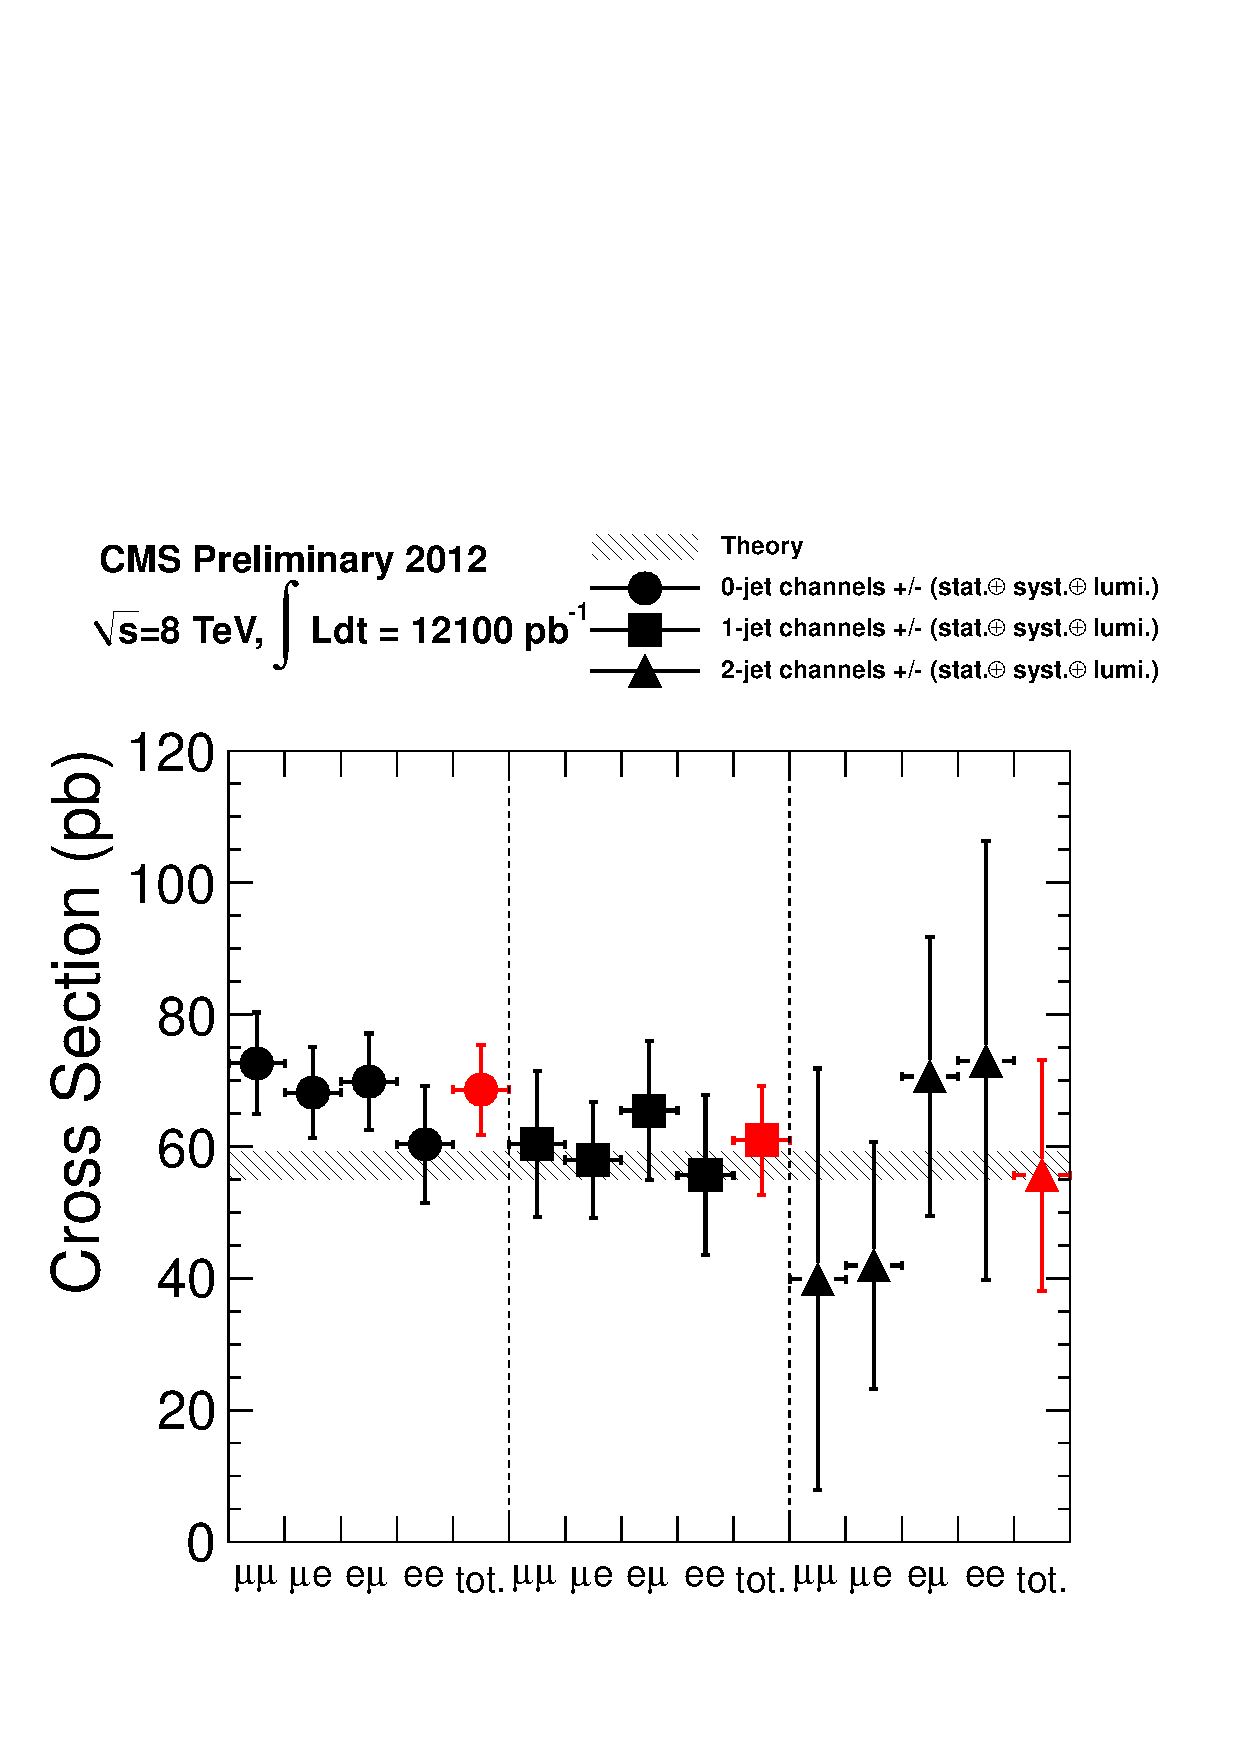
\includegraphics[width=.8\textwidth]{figures/ww_analysis20_0_summary.pdf}
\caption{Summary of all channels. Total uncertainty is shown.}
\label{fig:xs_summary_figure}
\end{figure}


\subsection{Control Plots for WW Cross Section}

%%%%%%%%%%%%%%%%%%%%
\begin{figure}[!hbtp]
\centering
\subfigure[\mll\ OF]{
\centering
\label{subfig:dilepmass_wwxsec_nj0_of.png}
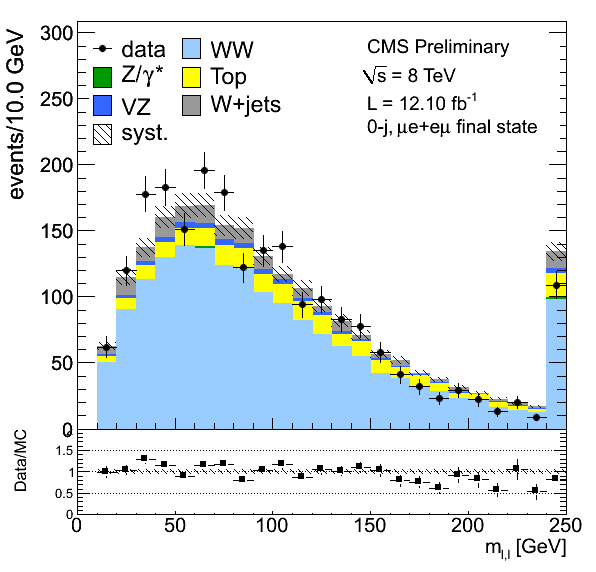
\includegraphics[width=.32\textwidth]{figures/dilepmass_wwxsec_nj0_of.png}
}
\subfigure[\mll\ SF]{
\centering
\label{subfig:dilepmass_wwxsec_nj0_sf.png}
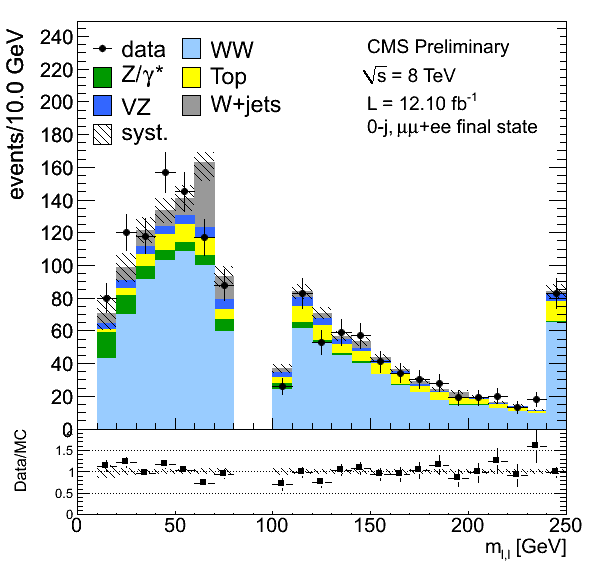
\includegraphics[width=.32\textwidth]{figures/dilepmass_wwxsec_nj0_sf.png}
}
\\
\subfigure[$m_T$ OF]{
\centering
\label{subfig:mt_wwxsec_nj0_of.png}
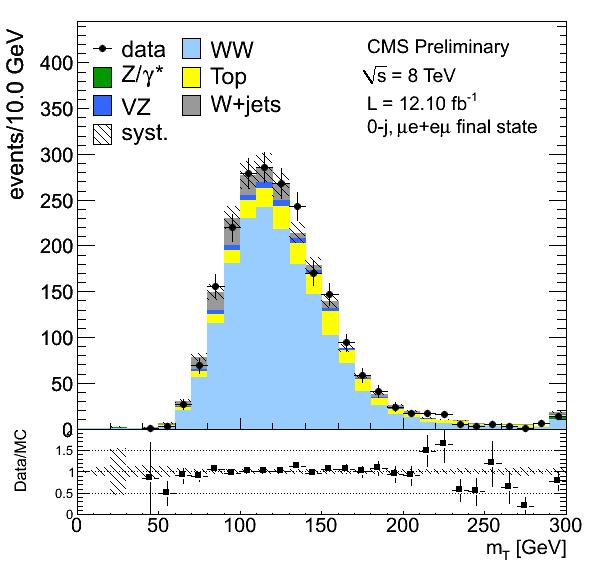
\includegraphics[width=.32\textwidth]{figures/mt_wwxsec_nj0_of.png}
}
\subfigure[$m_T$ SF]{
\centering
\label{subfig:mt_wwxsec_nj0_sf.png}
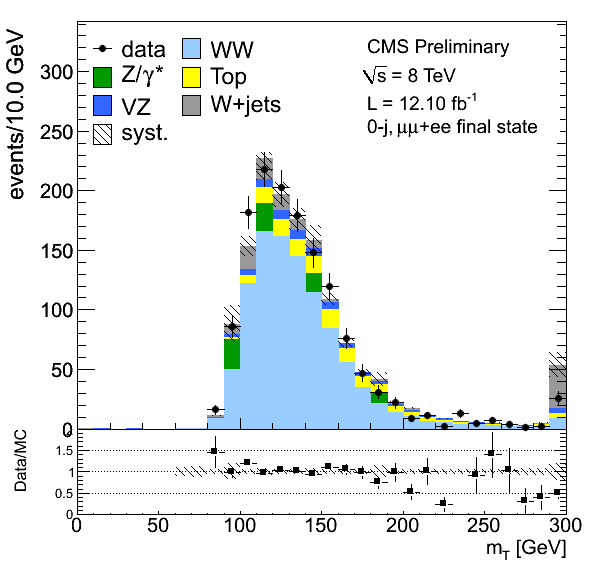
\includegraphics[width=.32\textwidth]{figures/mt_wwxsec_nj0_sf.png}
}
\\
\subfigure[\pt(l1) OF]{
\centering
\label{subfig:lep1pt_wwxsec_nj0_of.png}
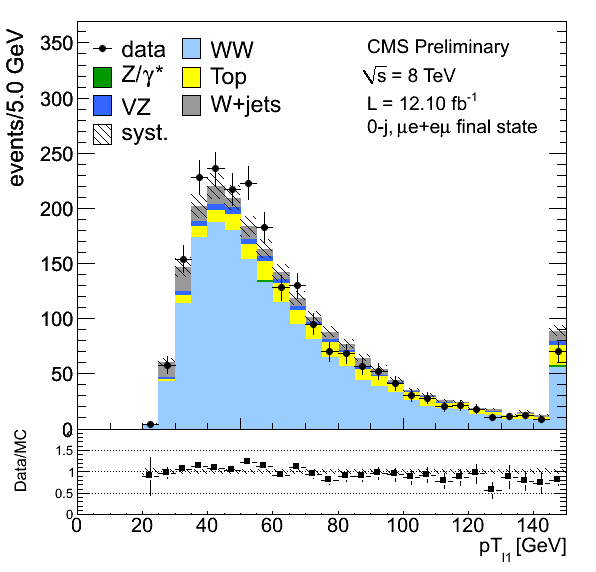
\includegraphics[width=.32\textwidth]{figures/lep1pt_wwxsec_nj0_of.png}
}
\subfigure[\pt(l1) SF]{
\centering
\label{subfig:lep1pt_wwxsec_nj0_sf.png}
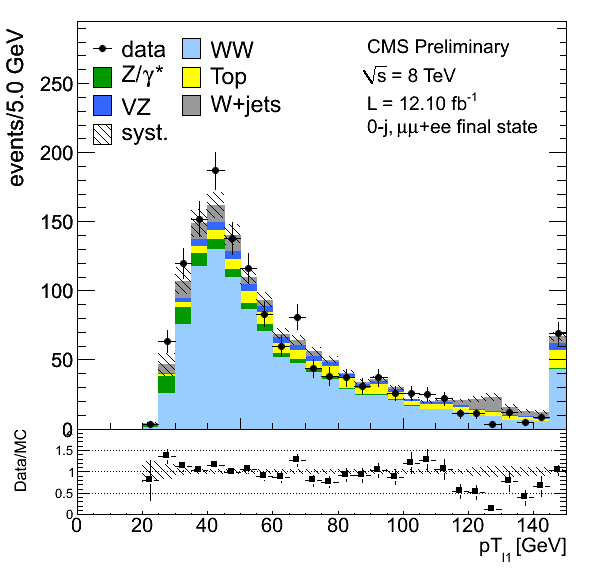
\includegraphics[width=.32\textwidth]{figures/lep1pt_wwxsec_nj0_sf.png}
}
\\
\subfigure[\pt(l2) OF]{
\centering
\label{subfig:lep2pt_wwxsec_nj0_of.png}
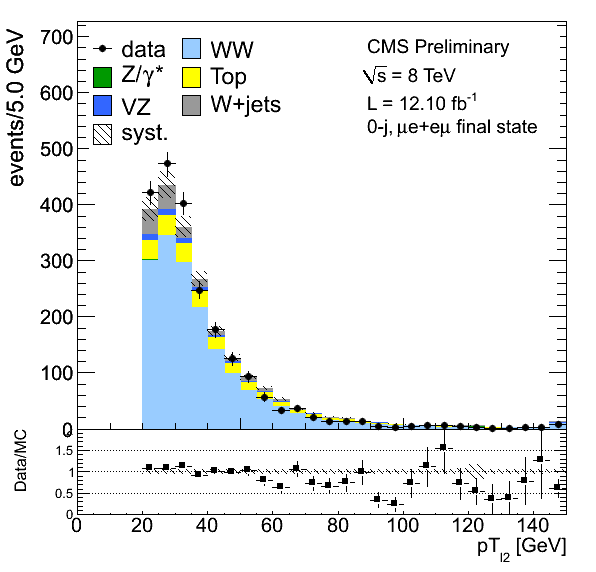
\includegraphics[width=.32\textwidth]{figures/lep2pt_wwxsec_nj0_of.png}
}
\subfigure[\pt(l2) SF]{
\centering
\label{subfig:lep2pt_wwxsec_nj0_sf.png}
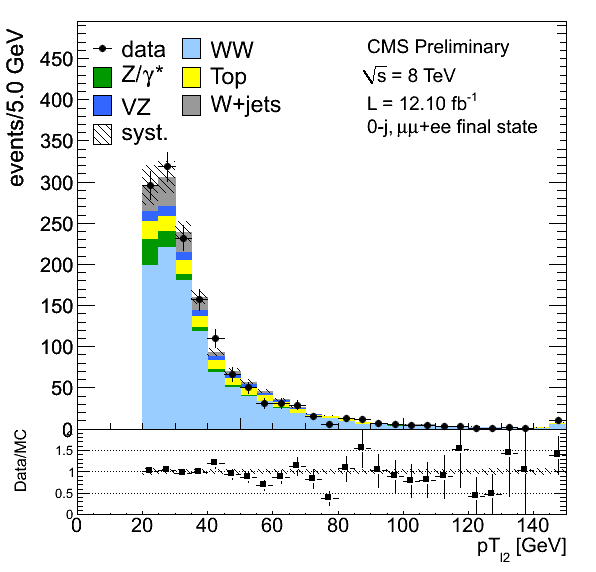
\includegraphics[width=.32\textwidth]{figures/lep2pt_wwxsec_nj0_sf.png}
}
\\
\caption{Control plots for WW cross section in 0-jet bin.}
\label{fig:wwxsec_nj0}
\end{figure}
%%%%%%%%%%%%%%%%%%%%

%%%%%%%%%%%%%%%%%%%%
\begin{figure}[!hbtp]
\centering
\subfigure[\mll\ OF]{
\centering
\label{subfig:dilepmass_wwxsec_nj1_of.png}
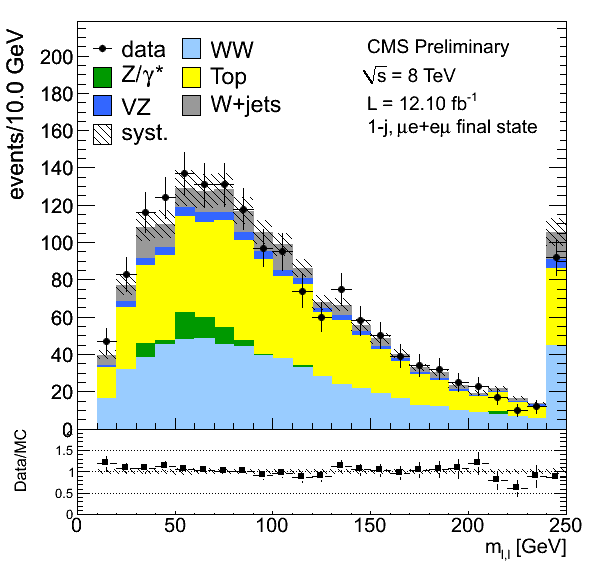
\includegraphics[width=.32\textwidth]{figures/dilepmass_wwxsec_nj1_of.png}
}
\subfigure[\mll\ SF]{
\centering
\label{subfig:dilepmass_wwxsec_nj1_sf.png}
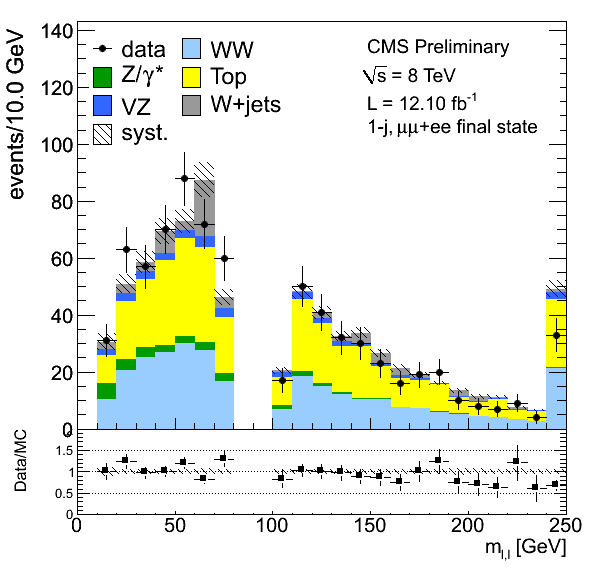
\includegraphics[width=.32\textwidth]{figures/dilepmass_wwxsec_nj1_sf.png}
}
\\
\subfigure[$m_T$ OF]{
\centering
\label{subfig:mt_wwxsec_nj1_of.png}
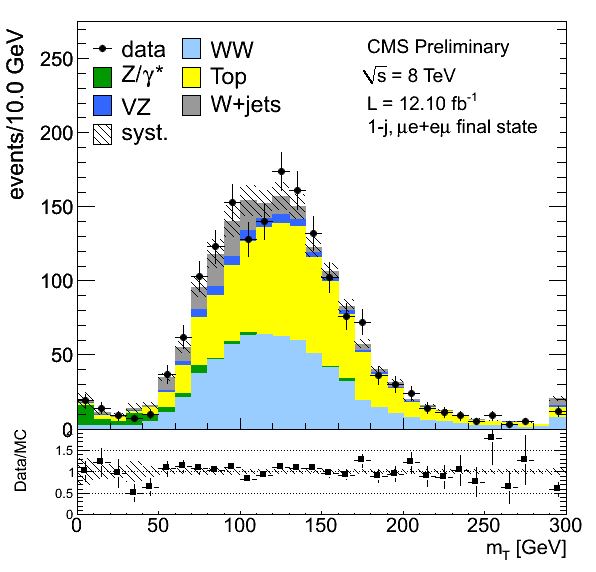
\includegraphics[width=.32\textwidth]{figures/mt_wwxsec_nj1_of.png}
}
\subfigure[$m_T$ SF]{
\centering
\label{subfig:mt_wwxsec_nj1_sf.png}
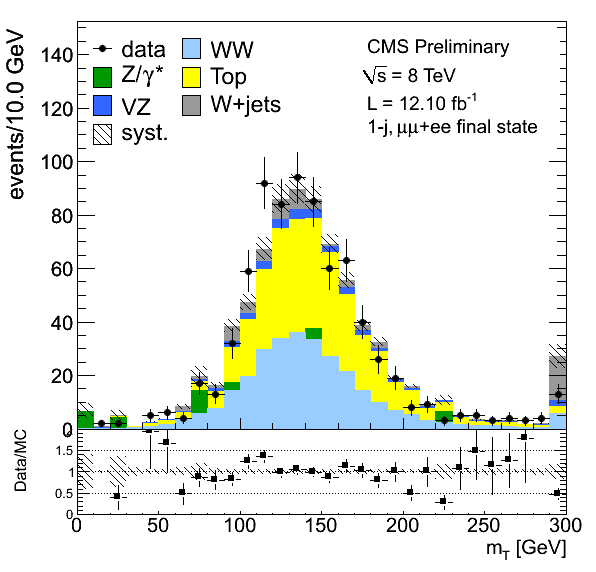
\includegraphics[width=.32\textwidth]{figures/mt_wwxsec_nj1_sf.png}
}
\\
\subfigure[\pt(l1) OF]{
\centering
\label{subfig:lep1pt_wwxsec_nj1_of.png}
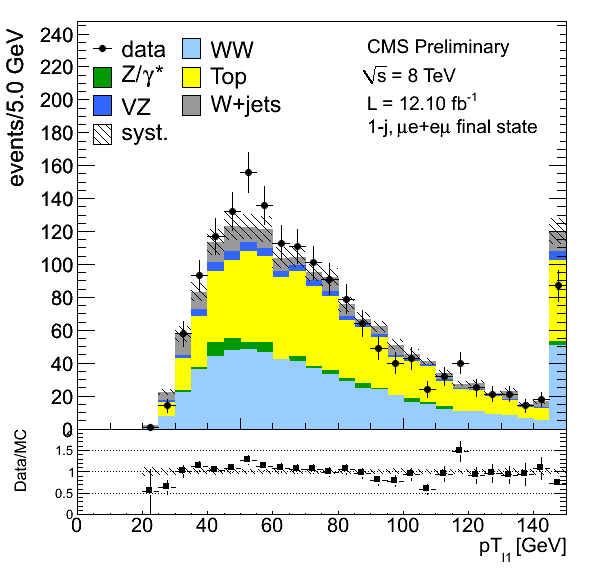
\includegraphics[width=.32\textwidth]{figures/lep1pt_wwxsec_nj1_of.png}
}
\subfigure[\pt(l1) SF]{
\centering
\label{subfig:lep1pt_wwxsec_nj1_sf.png}
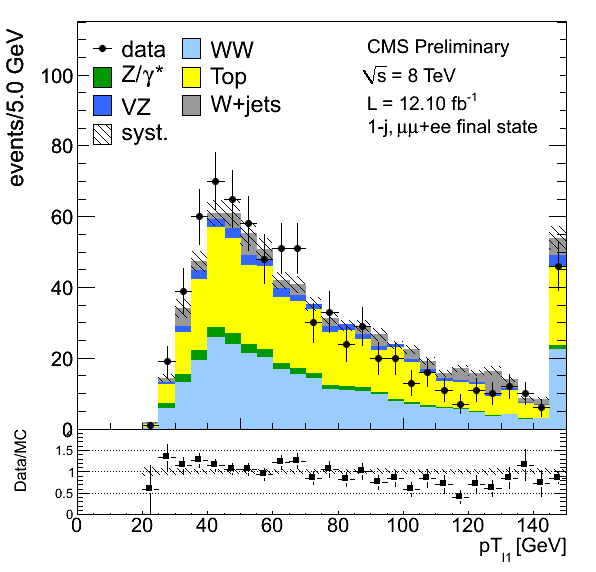
\includegraphics[width=.32\textwidth]{figures/lep1pt_wwxsec_nj1_sf.png}
}
\\
\subfigure[\pt(l2) OF]{
\centering
\label{subfig:lep2pt_wwxsec_nj1_of.png}
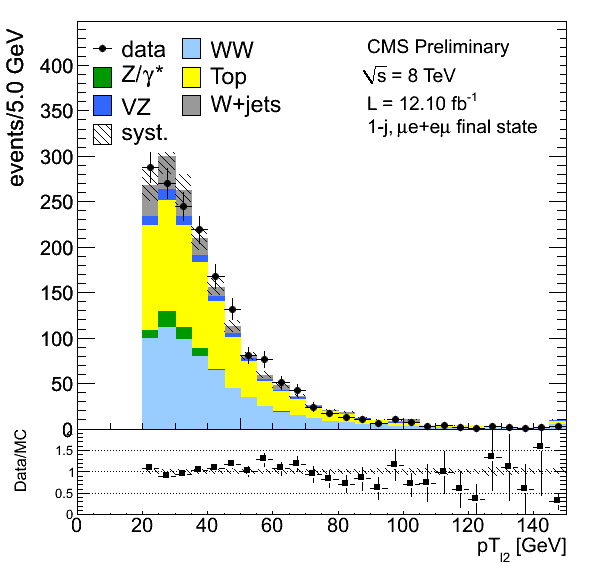
\includegraphics[width=.32\textwidth]{figures/lep2pt_wwxsec_nj1_of.png}
}
\subfigure[\pt(l2) SF]{
\centering
\label{subfig:lep2pt_wwxsec_nj1_sf.png}
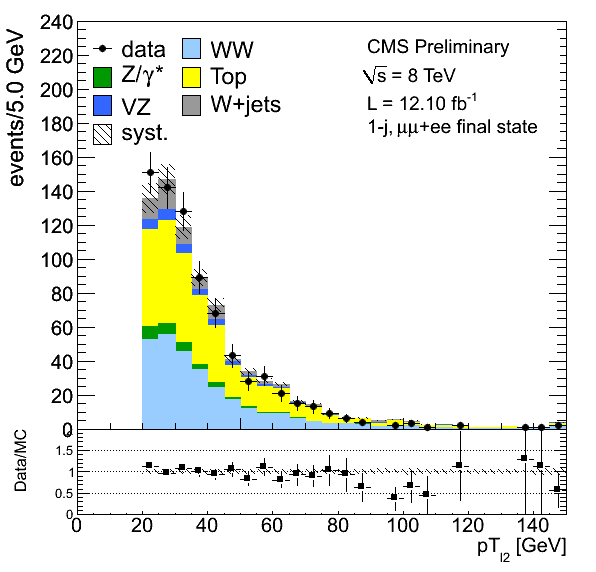
\includegraphics[width=.32\textwidth]{figures/lep2pt_wwxsec_nj1_sf.png}
}
\\
\caption{Control plots for WW cross section in 1-jet bin.}
\label{fig:wwxsec_nj1}
\end{figure}
%%%%%%%%%%%%%%%%%%%%

%%%%%%%%%%%%%%%%%%%%
\begin{figure}[!hbtp]
\centering
\subfigure[\mll\ OF]{
\centering
\label{subfig:dilepmass_wwxsec_nj2_of.png}
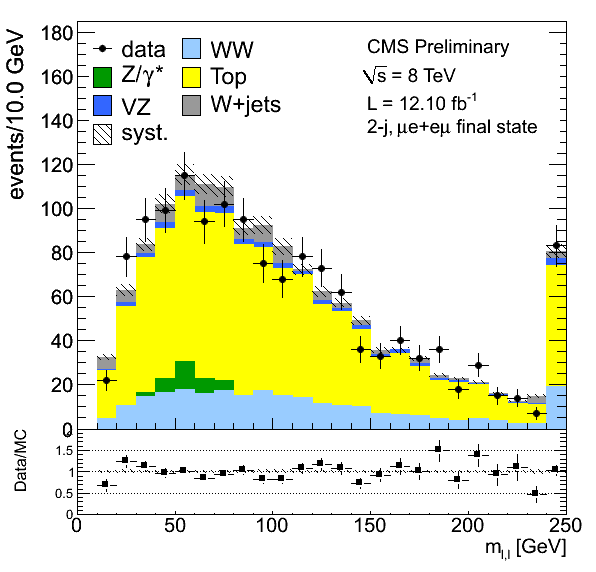
\includegraphics[width=.32\textwidth]{figures/dilepmass_wwxsec_nj2_of.png}
}
\subfigure[\mll\ SF]{
\centering
\label{subfig:dilepmass_wwxsec_nj2_sf.png}
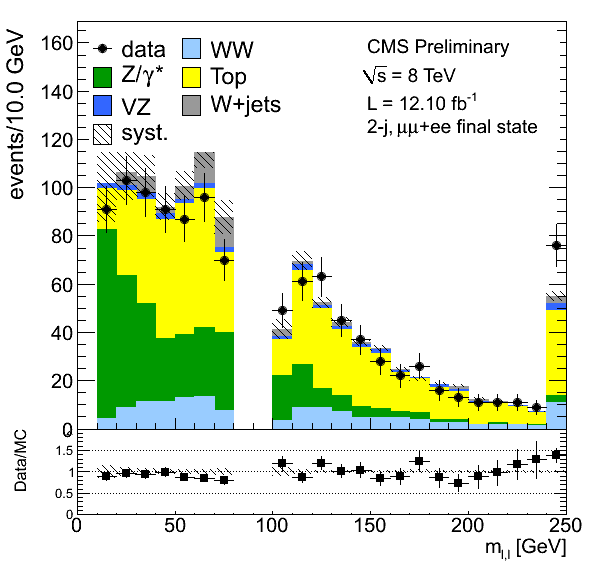
\includegraphics[width=.32\textwidth]{figures/dilepmass_wwxsec_nj2_sf.png}
}
\\
\subfigure[$m_T$ OF]{
\centering
\label{subfig:mt_wwxsec_nj2_of.png}
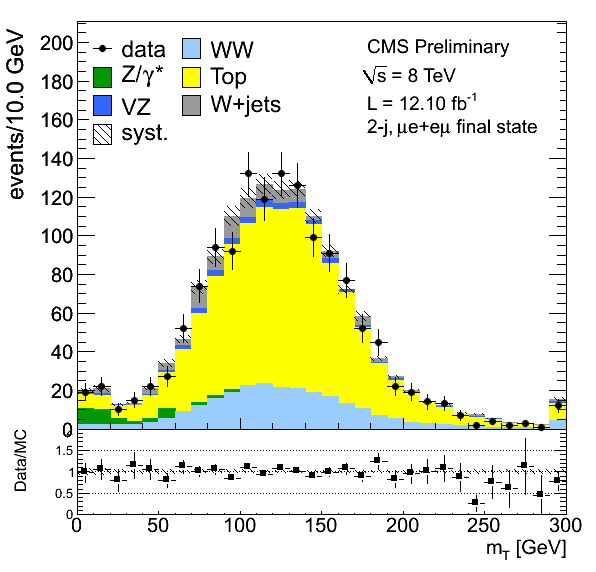
\includegraphics[width=.32\textwidth]{figures/mt_wwxsec_nj2_of.png}
}
\subfigure[$m_T$ SF]{
\centering
\label{subfig:mt_wwxsec_nj2_sf.png}
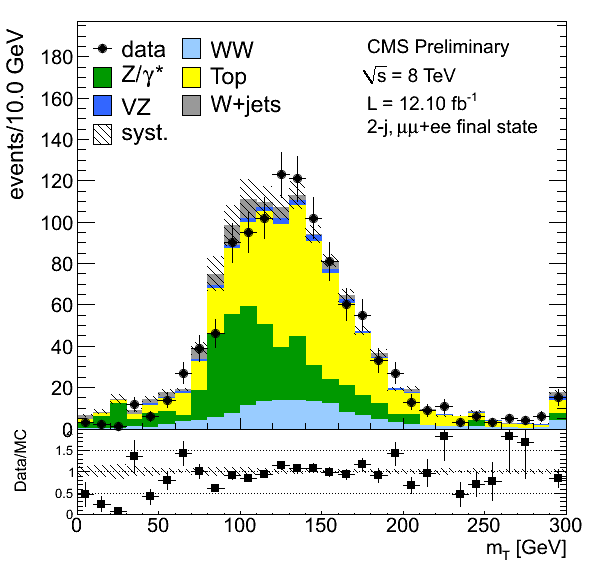
\includegraphics[width=.32\textwidth]{figures/mt_wwxsec_nj2_sf.png}
}
\\
\subfigure[\pt(l1) OF]{
\centering
\label{subfig:lep1pt_wwxsec_nj2_of.png}
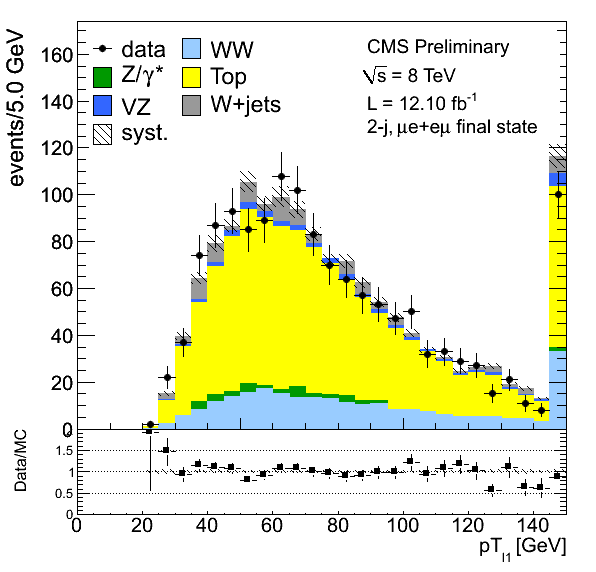
\includegraphics[width=.32\textwidth]{figures/lep1pt_wwxsec_nj2_of.png}
}
\subfigure[\pt(l1) SF]{
\centering
\label{subfig:lep1pt_wwxsec_nj2_sf.png}
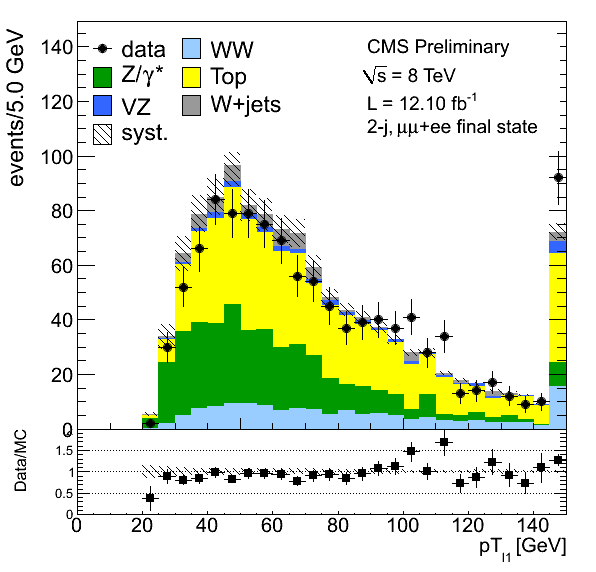
\includegraphics[width=.32\textwidth]{figures/lep1pt_wwxsec_nj2_sf.png}
}
\\
\subfigure[\pt(l2) OF]{
\centering
\label{subfig:lep2pt_wwxsec_nj2_of.png}
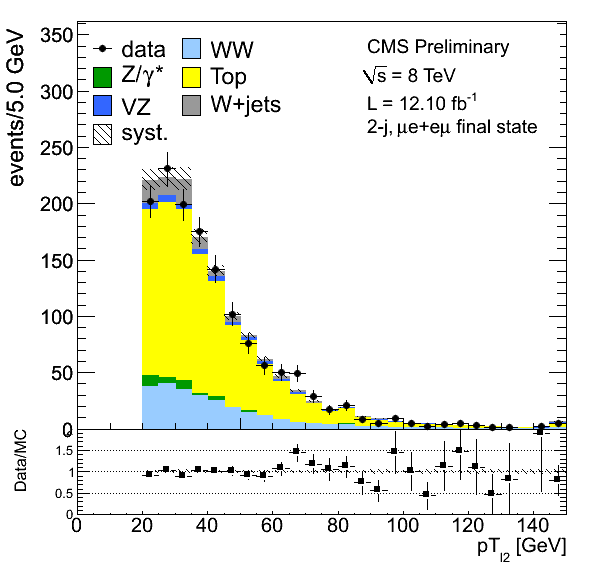
\includegraphics[width=.32\textwidth]{figures/lep2pt_wwxsec_nj2_of.png}
}
\subfigure[\pt(l2) SF]{
\centering
\label{subfig:lep2pt_wwxsec_nj2_sf.png}
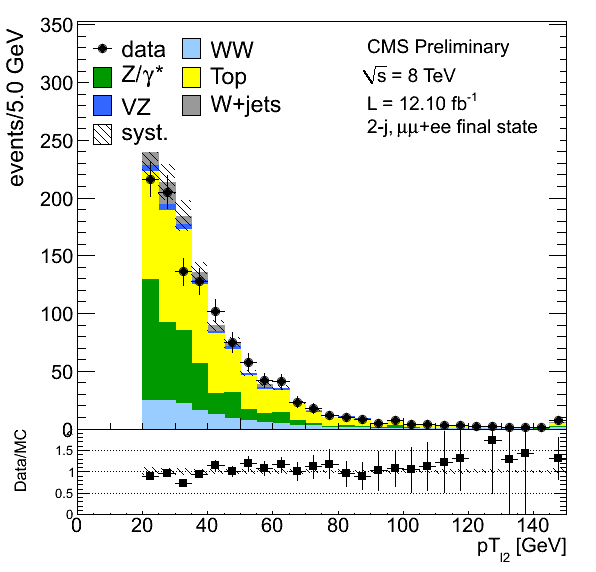
\includegraphics[width=.32\textwidth]{figures/lep2pt_wwxsec_nj2_sf.png}
}
\\
\caption{Control plots for WW cross section in 2-jet bin.}
\label{fig:wwxsec_nj2}
\end{figure}
%%%%%%%%%%%%%%%%%%%%
